\documentclass{article}

\usepackage{amsmath,graphicx,parskip,mathrsfs,subfigure}
\usepackage{fancyhdr}
\usepackage{amsthm,amssymb}
\usepackage{setspace}
\usepackage{epstopdf}
\usepackage{hyperref}
\usepackage[left=3cm,right=3cm,top=3cm,bottom=3cm]{geometry}

\pagestyle{fancy}
\lhead{Samuel Huberman}
\chead{MSE1022:HW3C}
\rhead{999157923}

\begin{document}
\begin{figure}[h!]
\centering
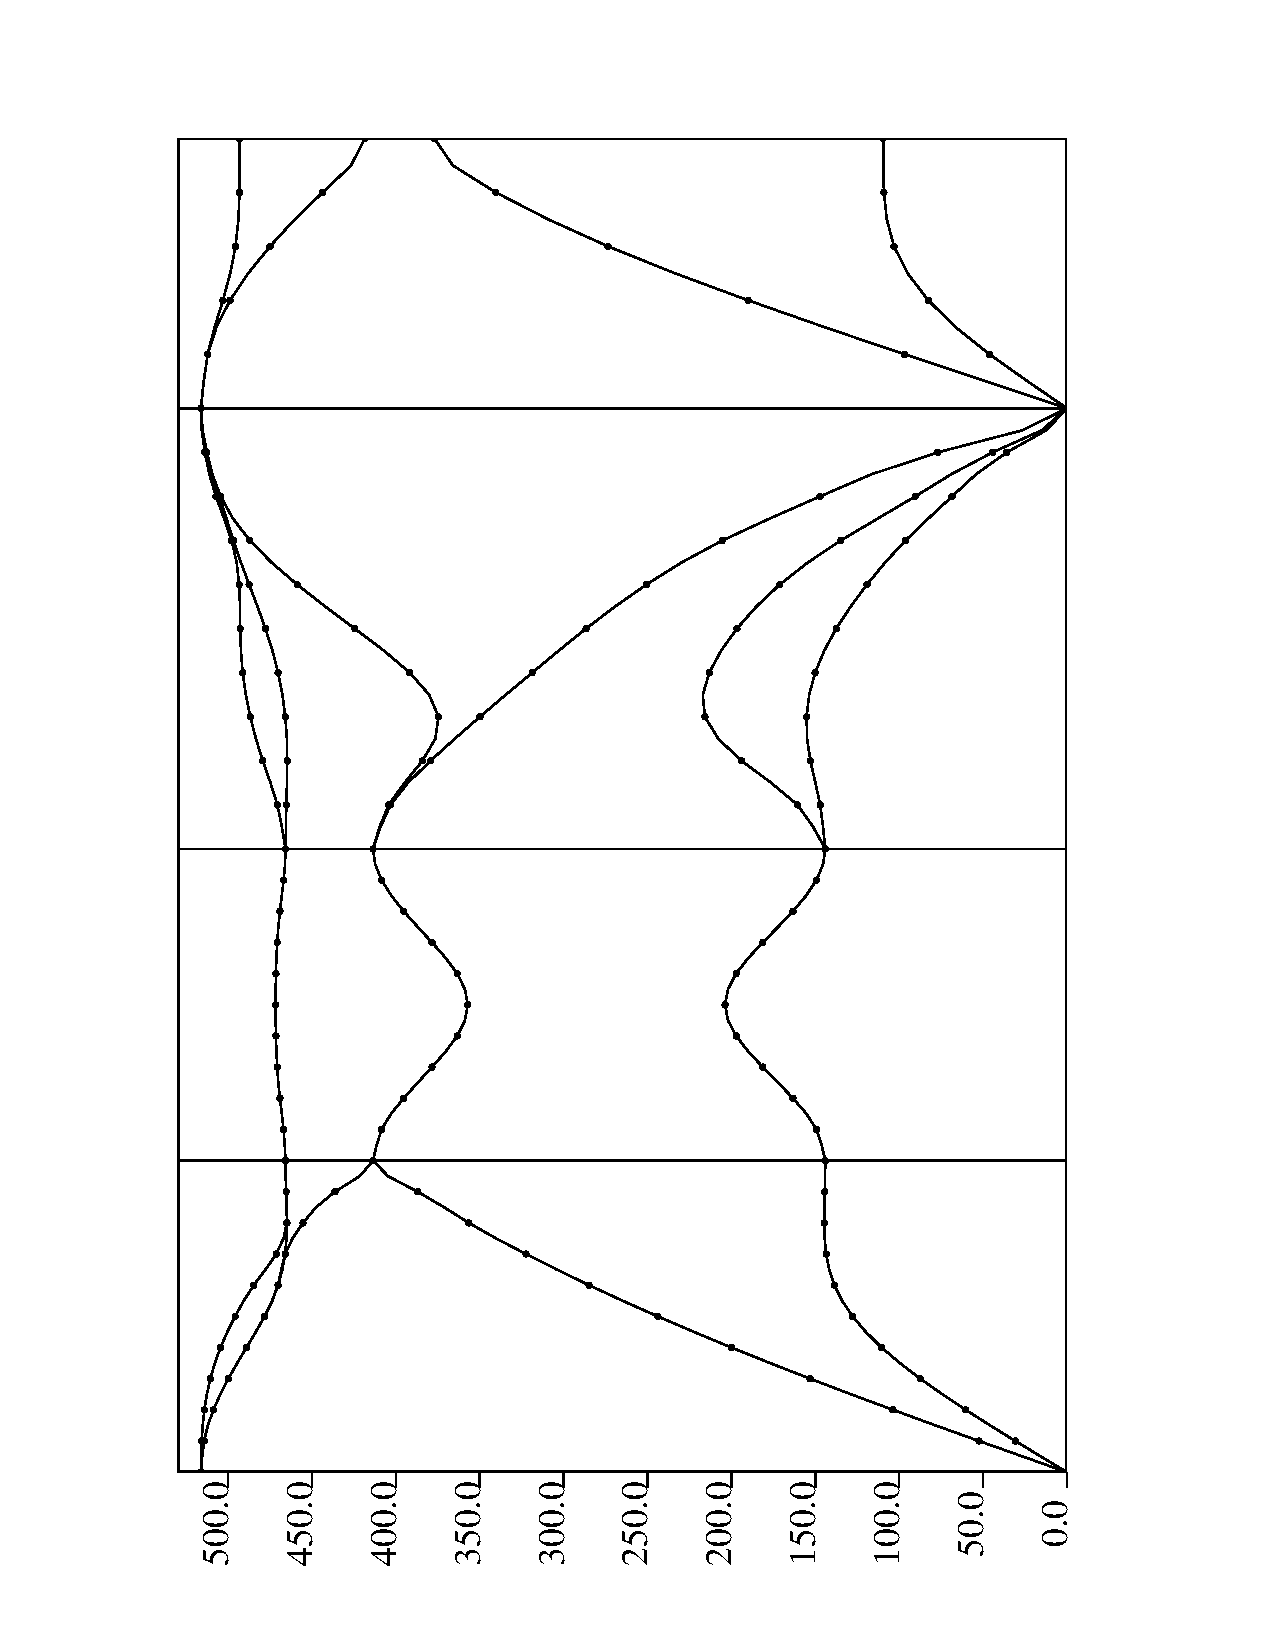
\includegraphics[scale=0.4, angle=-90]{siph}
\caption{Silicon Dispersion from DFPT; y-axis is frequency in [$cm^{-1}$], vertical lines are high symmetry points in BZ, from left to right $\Gamma$, $X$, $K$, $\Gamma$, $L$}
\end{figure}
\begin{figure}[h!]
\centering
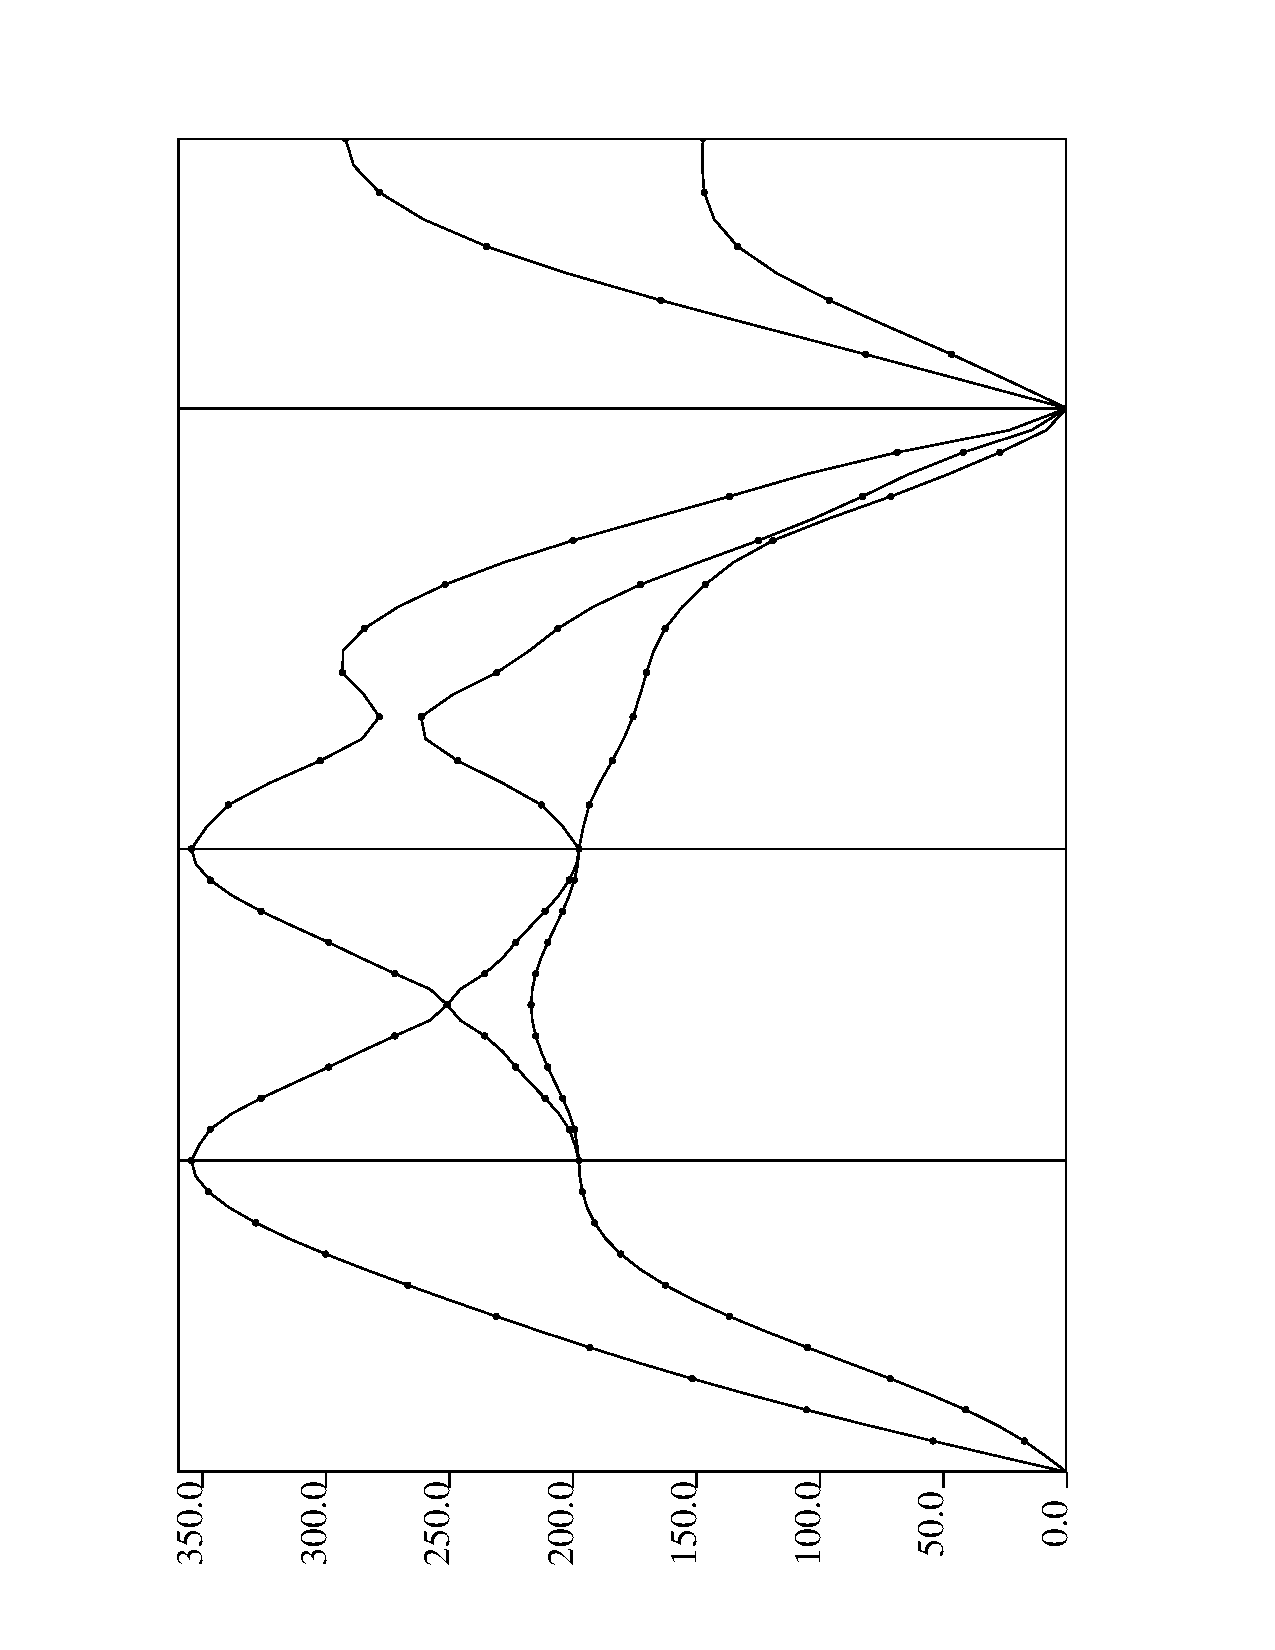
\includegraphics[scale=0.4, angle=-90]{alph}
\caption{Aluminium Dispersion from DFPT; y-axis is frequency in [$cm^{-1}$], vertical lines are high symmetry points in BZ,from left to right $\Gamma$, $X$, $K$, $\Gamma$, $L$}
\end{figure}
Unlike the calculation of the electronic band structure, the phonon dispersions from DFPT are in excellent agreement with experimental data obtained from inelastic neutron scattering (Silicon from Dolling in 1963 and Aluminum from Stedman in 1966)  because of the relative ease with which accurate interatomic force constants can be determined (electron orbitals from DFT remain amibiguous). The extra branches present in Silicon and absent in Aluminum are the consequence of the extra atom present in the primitive cell of the diamond crystalline structure.

\begin{figure}[h!]
\centering
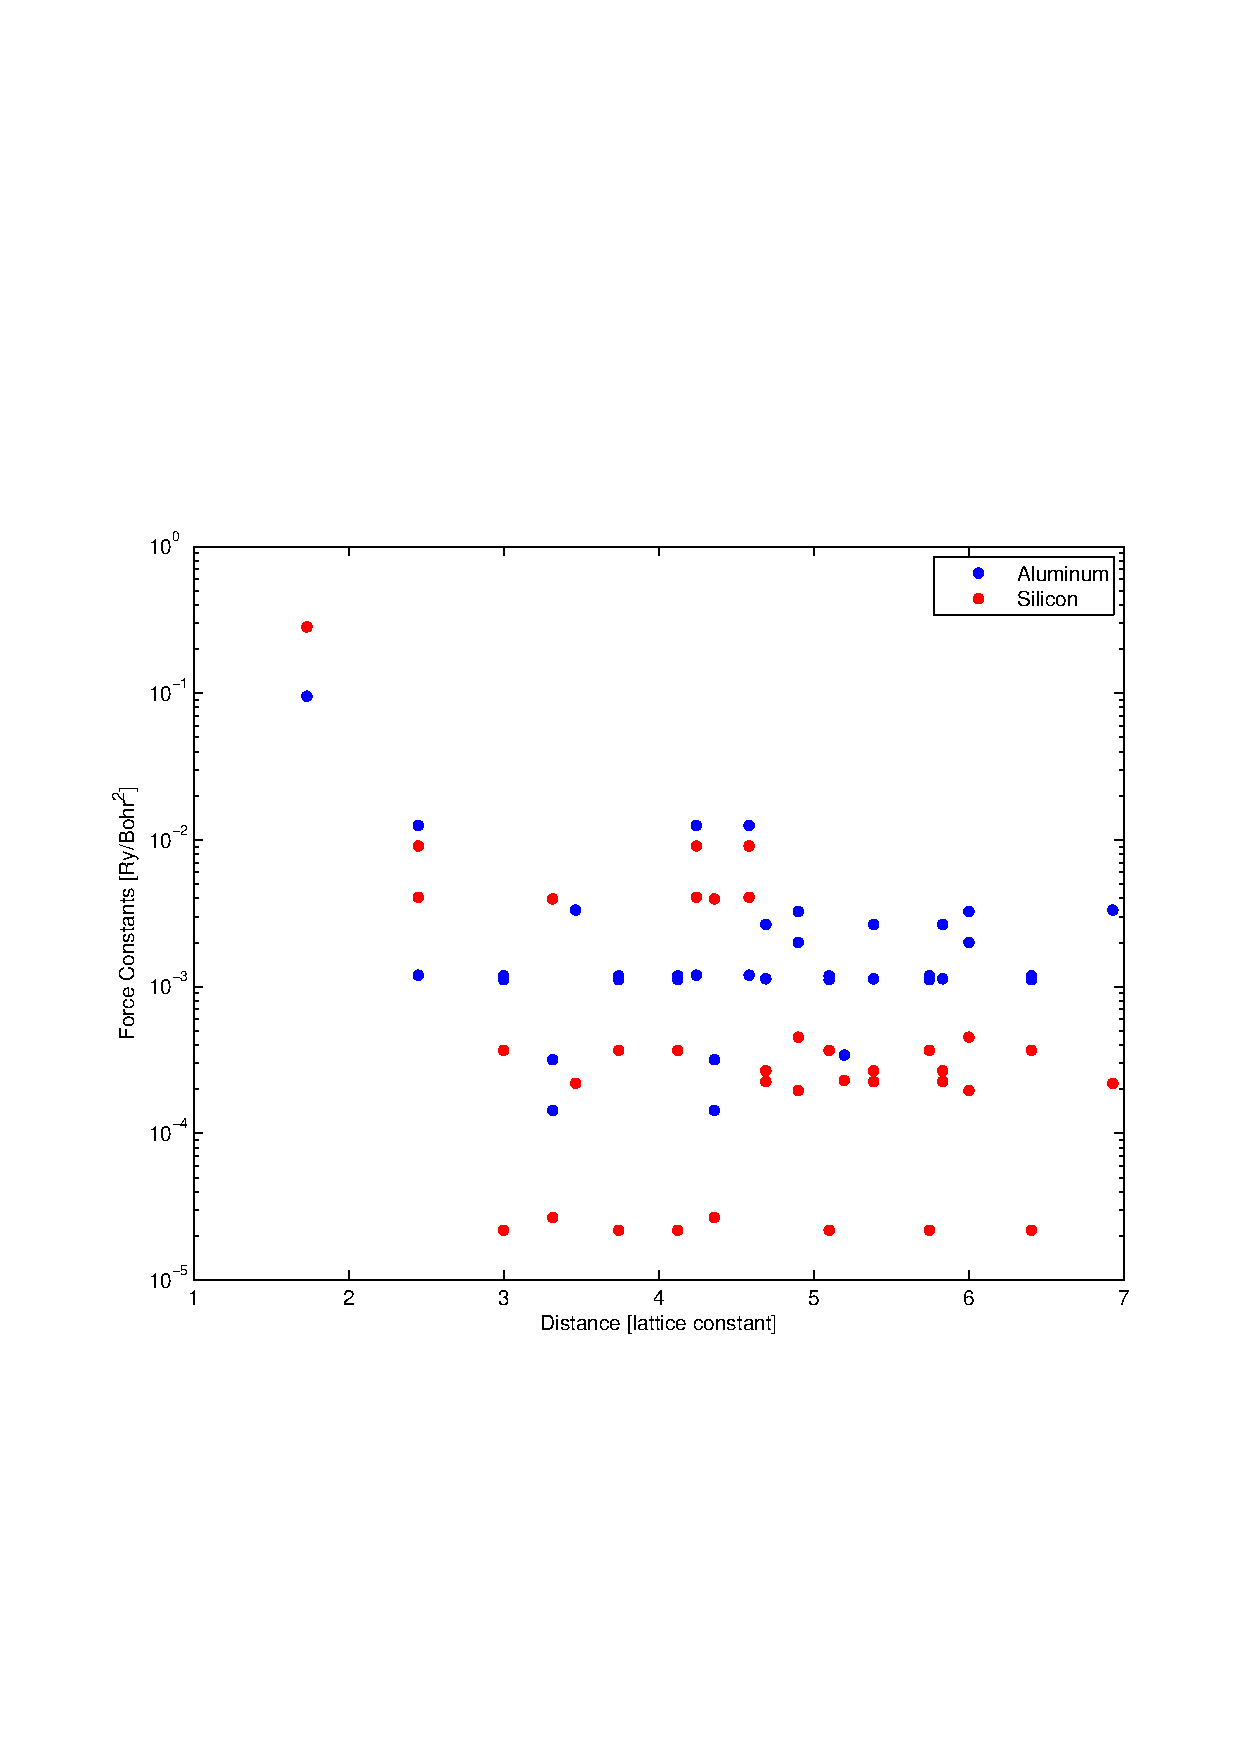
\includegraphics[scale=0.5]{fc}
\caption{Selected harmonic force constants}
\end{figure}
\end{document}

